\section{Regression Trees}
The predictors which are most frequently used in combination with Bagging are Classification and Regression Trees. We focus on Regression Trees, which are used to predict a numerical response variable.\footnote{Although tree-based methods are most frequently used for classification problems we want to restrict our attention to Regression Trees. In classification settings problems arise which are not essential to the analysis of Bagging. An example is the proper choice of accuracy  measure. In a regression setup, the residual sum of squares is used, but this measure is not suitable for classification. Here the best choice of measure is not clear.} Although Regression Trees exhibit a low bias, they are not competitive to other prediction methods as they react sensitive to changes in the data and therefore have a large variance. In combination with Bagging and its variance reducing effect bagged Regression Trees provide a powerful tool for prediction. The formal presentation of Regression Trees follows \cite{EoSL}. For a detailed treatment of Regression Trees implemented with the CART algorithm see \cite{Breiman1984}.

\noindent
\subsection{Prediction using Regression Trees}\label{sec:Tree_Pred}
Consider the following setting. Assume we are interested in the prediction of a continuous response variable denoted as $y$ on the basis of a set of $p$ explanatory variables $\mathbf{x}=(x_1,x_2,...,x_p)^T$. Furthermore, assume our data consists of $n$ observations, so we have $L_i = (y_i,\mathbf{x}_i)$ for data instances $i=1,...,n$. The setting and denotations carry over to subsequent sections.\\
A Regression Tree model consists of a sequence of binary decision rules, which can be summarized in a tree diagram. A decision rule is defined by an explanatory variable (splitting variable) and a value in the domain of the respective variable (split point). We refer to decision rules as nodes. An exemplary Regression Tree for a two-dimensional predictor space $\mathbf{x}=(x_1,x_2)^T \in [0,1]^2$ is provided in Figure \ref{fig:Tree_FigTreePar} (a).

\begin{figure}[htb]
\centering
\begin{minipage}[c]{.45\linewidth}
\centering
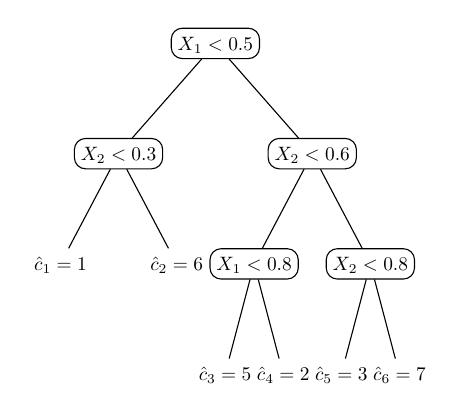
\begin{tikzpicture}[
scale = 0.7,
every node/.style={transform shape},
baseline,
level distance=20mm,
text depth=.1em,
text height=.8em,
level 1/.style={sibling distance=10em},
level 2/.style={sibling distance=6em},
level 3/.style={sibling distance=3em}]


	\node [rounded corners, draw] {$X_1 < 0.5$}
		child {node [rounded corners, draw] {$X_2 < 0.3$}
			child {node {$\hat{c}_1=1$}}
			child {node {$\hat{c}_2=6$}}
		}
		child {node [rounded corners, draw] {$X_2 < 0.6$}
			child {node [rounded corners, draw] {$X_1<0.8$}
				child {node {$\hat{c}_3=5$}}
				child {node {$\hat{c}_4=2$}}
			}
			child {node [rounded corners, draw] {$X_2<0.8$}
				child {node {$\hat{c}_5=3$}}
				child {node {$\hat{c}_6=7$}}
			}
	};

\end{tikzpicture}
\subcaption{Illustration Regression Tree}
\end{minipage}%
\hfill%
\begin{minipage}[c]{.45\linewidth}
\centering
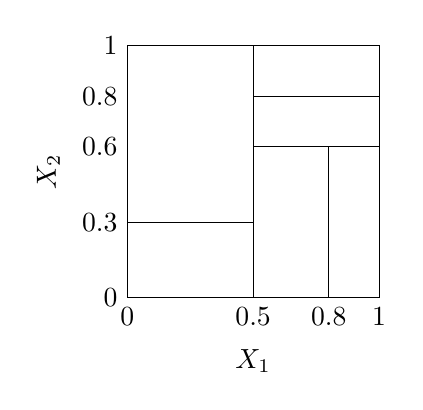
\begin{tikzpicture}[scale = 0.8]

\draw (0,0) -- (4,0) -- (4,4) -- (0,4) -- (0,0);
\draw (2,0) -- (2,4);
\draw (0,1.2) -- (2,1.2);
\draw (2,2.4) -- (4,2.4);
\draw (2,3.2) -- (4,3.2);
\draw (3.2,0) -- (3.2,2.4);
\node [left] at (0,0) {0};
\node [left] at (0,1.2) {0.3};
\node [left] at (0,2.4) {0.6};
\node [left] at (0,3.2) {0.8};
\node [left] at (0,4) {1};
\node [below] at (2,0) {0.5};
\node [below] at (0,0) {0};
\node [below] at (4,0) {1};
\node [below] at (3.2,0) {0.8};
\node[rotate=90] at (-1.25,2) {$X_2$};
\node at (2,-1) {$X_1$};
\end{tikzpicture}
\subcaption{Illustration Partition}
\end{minipage}
\caption[Illustration of a Regression Tree and its corresponding Partition]{Illustration of a Regression Tree and its corresponding Partition}
\label{fig:Tree_FigTreePar}

\end{figure}


\noindent
A prediction for a new observation $\mathbf{x^{new}}$ is obtained by following down the tree diagram, starting at the top node. At each node continue on the left branch if the decision rule is satisfied and on the right if not. This procedure is continued until a final branch of the tree diagram is reached. We refer to final branches as terminal nodes and to the number of final branches as size of the Tree. Each terminal node is labeled with a constant $\hat{c}_k$ with $k \in \{1,...,6\}$. This constant is used as predicted value for an observation $\mathbf{x^{new}}$ reaching the corresponding terminal node. For instance, the prediction for an exemplary observation $\mathbf{x^{new}}=(0.4,0.4)^T$ using the Regression Tree of Figure~\ref{fig:Tree_FigTreePar}~(a) is $\hat{c}_2=6$.

\subsection{The CART Algorithm}
The method which is most widely used to construct Regression Trees is the so-called Classification and Regression Tree (CART) algorithm developed by \cite{Breiman1984}. The basic idea of the procedure is to group data with similar characteristics. For this, the CART algorithm partitions the feature space (spanned by $x_1, ..., x_p$) by successive binary splits. These binary splits correspond to the decision rules of the tree diagram. Each terminal node corresponds to a region in the partition and the corresponding constant is used as predicted value for an observation falling into the respective region. A graphical illustration of the two-dimensional example is provided in Figure \ref{fig:Tree_FigTreePar} (b).

Repeated binary splits are a reasonable simplification as the determination of the best binary partition is computational infeasible\footnote{The best binary partition would require to calculate for any sequence of binary splits and any possible split point at each node the residual sum of squares of the resulting predictor, which is computationally infeasible.} (see Hyafil and Rivest (1976)). The CART algorithm is computational feasible, as the determination of the split point can be done quickly and the procedure has to be repeated for only $p$ input variables (Hastie et al. (2009, p.307)). However, this procedure might not result in the best binary partition.\\


\noindent
The CART algorithm works as follows. In the first step, the entire feature space is split at split point $d$, using splitting variable $x_j$ ($j \in \{1,...,p\}$), into two regions denoted as $R_1$ and $R_2$. Equivalently we can think of dividing the entire data set into two subsets. These regions are defined as
$$R_1(j,d)=\{\mathbf{x}|x_j \le d\} \text{ and } R_2(j,d)=\{\mathbf{x}|x_j > d\}.$$
\noindent
Split point $d$ and splitting variable $x_j$ are chosen such that the residual sum of squares is minimized in the resulting regions. This means $d$ and $x_j$ are chosen such that following minimization problem is solved.
\begin{equation}
\label{eq:CARTmin}
\min\limits_{j,d}[\min\limits_{c_1}\sum\limits_{\mathbf{x_i} \in R_1(j,d)}(y_i-c_1)^2 + \min\limits_{c_2}\sum\limits_{\mathbf{x_i} \in R_2(j,d)}(y_i-c_2)^2]
\end{equation}
\noindent
The inner minimization problem determines the best choice (in terms of residual sum of squares) of the constants in the resulting regions. The best choice is simply the sample average of observations in the respective region (Breiman et al. (1984, p. 230)). The outer minimization problem selects the optimal split point and the optimal splitting variable. To solve this problem we determine for each splitting variable the optimal split point and then select the splitting variable yielding the lowest residual sum of squares. We denote the optimal choice of splitting point by $d^0$ and the optimal constant by $c^0$. Estimates are denoted as $\hat{d}$ and $\hat{c}$, respectively. In the next step the CART algorithm considers the resulting regions and applies the same procedure to them. Therefore the method is known as \textit{binary recursive splitting}.  The procedure is repeated until a stopping rule is satisfied, for instance if a minimum amount of observations in each terminal node is achieved. An alternative stopping rule prescribes to add further nodes as long as the next node reduces residual sum of squares by a predetermined amount.

Now consider a partition of the feature space into $K$ regions $R_1,...,R_K$. The regression function for this partition can be expressed as follows
\begin{equation}
\label{eq:CARTpred}
\hat{\theta}(\mathbf{x})= h_{n}(L_{1},\dots, L_{n})(\mathbf{x})=\sum\limits_{k=1}^{K}\hat{c}_k\mathbbm{1}_{[\mathbf{x}\in R_k]},
\end{equation}
where the function  $h_n:\mathbb{R}^{p} \rightarrow \mathbb{R}$ is the CART algorithm.\\
Similarly to the solution to the inner minimization problem of \eqref{eq:CARTmin} the optimal choice for the constant is given by the sample average of observations in the respective region (Breiman et al. (1984, p.230)). Expression \eqref{eq:CARTpred} reveals that the true data generating process is approximated by a piecewise constant step function.

\subsection{Bias-Variance Tradeoff} \label{sec:BiasVariance}
Breiman et al. (1984, p.272) state that any further node will never increase the (expected) sum of squared errors. This means that any further split will (weakly) improve the fit to the initial data set. For instance, if we grow a Tree to its maximal size, i.e. until only one observation is left in each terminal node, the initial data set is fit identically. The number of terminal nodes is governed by stopping rules. Consequently, stopping rules influence the flexibility of the regression function to adapt to the data set.

First consider a stopping rule which allows for large Regression Trees. These models can adapt flexibly to any complex true relationship in the data and will therefore exhibit a low bias. The problem with this adaptiveness is the risk of fitting the artificial noise in the data (overfitting). Fitting the artificial noise of the data will result in a sensitivity to changes in the data, i.e. a high variance. In contrast, if we select a more restrictive stopping rule we might not capture the fundamental relationships in the data (underfitting). However, this procedure will be more robust to changes in the data. In conclusion we encounter a tradeoff between bias and variance in the specification of Regression Tree models, which is governed by stopping rules.\footnote{This trade-off between bias and variance is not specific to Regression Trees but rather a common problem in statistical modeling.}

\subsection{Instability}\label{sec:stability}
Regression Trees react particularly sensitive to changes in the data. Consider a small perturbation of the initial data set and assume this small perturbation already leads to a change of the split point or splitting variable at a top node. Due to the recursive structure all decisions followed by this node are affected as well. Therefore the change in the data will have a large impact on the resulting predictor (Breiman et al. (1984, p.156-159)). A graphical illustration of the instability of Regression Trees is provided in Appendix \ref{sec:instability}. \cite{Breiman1996} denote predictors for which a small perturbation in the data set leads to significant changes in the predictor as instable. The instability of Regression Trees is pointed out by \cite{breiman1996B}. For the theoretical analysis of Bagging a formal definition of the notion of instability is required. \cite{Buhlmann2002} provide the following definition which is not inconsistent with the heuristic definition by \cite{breiman1996B}.

\begin{definition}[Stability of a predictor] \label{stability}
A statistic $\hat{\theta}_{n}(\mathbf{x}) = h_{n}(L_{1},\dots, L_{n})(\mathbf{x})$ is called stable at $\mathbf{x}$ if $\hat{\theta}_{n}(\mathbf{x}) = \theta(\mathbf{x}) + o_{p}(1) \: (n \rightarrow \infty)$ for some fixed value $\theta(\mathbf{x})$.
\end{definition}

\noindent
This definition resembles the definition of consistency. The crucial difference is that the statistic $\hat{\theta}_n(\mathbf{x})$ does not need to converge to the true population parameter, but only to a stable limit $\theta$. This means that an unstable predictor will assume a different limit value for another data set (taken from the same data generating process) with positive probability, even if the size of the data set goes to infinity.
